\documentclass{article}
\usepackage[margin=1in]{geometry}
\usepackage{amsmath,amsthm,amssymb}
\usepackage{bbm,enumerate,mathtools}
\usepackage{tikz,pgfplots}
\usepackage{chessboard}
\usepackage[hidelinks]{hyperref}
\usepackage{multicol} % Problem 35

\newenvironment{question}{\begin{trivlist}\item[\textbf{Question.}]}{\end{trivlist}}
\newenvironment{note}{\begin{trivlist}\item[\textbf{Note.}]}{\end{trivlist}}
\newenvironment{references}{\begin{trivlist}\item[\textbf{References.}]}{\end{trivlist}}
\newenvironment{related}{\begin{trivlist}\item[\textbf{Related.}]\end{trivlist}\begin{enumerate}}{\end{enumerate}}


\begin{document}
\rating{2}{1}
Say that a number $M$ is $(n, k)$-constructible if there exists an $n\times n$
board with $M$ $k$-in-a-row markers.
\begin{figure}[!h]
  \centering
  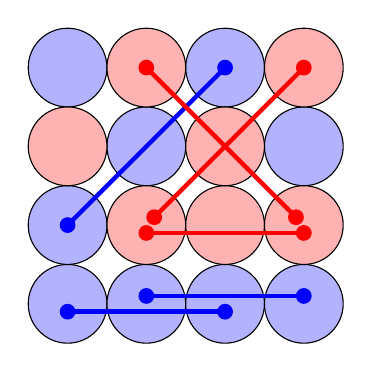
\begin{tikzpicture}
    \foreach \x/\y in {0/0,0/1,0/3,1/0,1/2,2/0,2/3,3/0,3/2} { \draw[fill=blue!30] (\x,\y) circle (0.5cm); }
    \foreach \x/\y in {0/2,1/1,1/3,2/1,2/2,3/1,3/3} { \draw[fill=red!30] (\x,\y) circle (0.5cm); }
    \foreach \x/\y/\a/\b in {0/1/2/3,0/-0.1/2/-0.1,1/0.1/3/0.1} {
      \draw[ultra thick, blue] (\x,\y)--(\a,\b);
      \fill[blue] (\x, \y) circle (0.1cm);
      \fill[blue] (\a, \b) circle (0.1cm);
    }
    \foreach \x/\y/\a/\b in {
      1/3/2.9/1.1,
      1.1/1.1/3/3,
      1/0.9/3/0.9}
    {
      \draw[ultra thick, red] (\x,\y)--(\a,\b);
      \fill[red] (\x, \y) circle (0.1cm);
      \fill[red] (\a, \b) circle (0.1cm);
    }
  \end{tikzpicture}
  \caption{
    The number $6$ is $(4, 3)$-constructible because the above $4 \times 4$
    board has $6$ sets of markers that are placed $3$-in-a-row.
    (This figure was borrowed from Problem 45.)
  }
\end{figure}
\begin{question}
  What is a procedure for determining if a grid has a solution? If it has a
  unique solution?
\end{question}
\begin{related}
  \item What if there are $\ell$ colors of pieces?
  \item What numbers have the greatest number of constructions? Up to dihedral
    action?
  \item What is the smallest number that is $(n, k)$-constructible?
  \item What if this is done on a hypercube or a triangular grid?
\end{related}
\begin{references}
  \item Problem 45.
\end{references}

\end{document}
